\subsection{Real time}\label{RealTime}

Real time (or stream) processing is used when there are multiple sources feeding data all the time \parencite{wu2020reactive}.

Real world example could be water slide. There is a queue of people waiting for the ride. Operator approves each person to take a ride one after the other.  

Similarly, in stream processing, computer (server) is always waiting and ready for the files to be uploaded. We can get 1 or n number of files per second, all of them will be send to our pipeline. For example, IoT sensors. They are constantly sending the data in order to extract relevant information.

In our case, if game would be played online we would use real time operation. This is due to player movements. The rough concept would be for player to make a move, that is recorded in database and with API we would constantly getting new, updated information.


\begin{figure}[H]
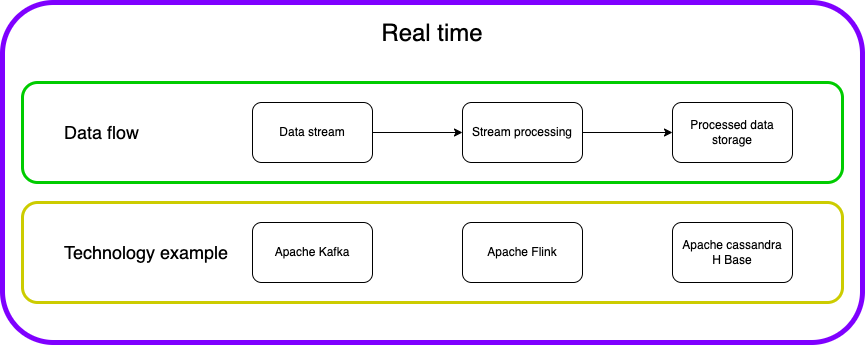
\includegraphics[scale=0.45]{img/ProcessingParadigms/BigData-RealTime.png}
\centering
\caption{Real time}
\label{fig:RealTime}
\end{figure}